\chapter{Analyse}

I dette kapitel vil vi gennemgå kravspecifikation til programmet, samt optegne og forklare forskellige modeller.


\section{Kravspecifikation}

Herunder ses en liste over krav til spillet, udformet udfra opgavebeskrivelsen \& det udleverede regelsæt.\footnote{Enkelte krav er hentet fra tidligere CDIO2-rapport af samme gruppe.}

\subsubsection{Alle krav stillet}

\begin{enumerate}
\item Der skal oprettes forskellige typer felter, samt en spilleplade.
\item Hvert felt skal påvirke spillernes pengebeholdning forskelligt, og have en udskrift om hvilket felt han ramte.
\item Spillerne skal kunne lande på et felt, og fortsætte derfra på næste slag.

\item Spillerne skal gå i ring rundt på felterne, på spillepladen, med uret. (man kan ikke gå mod uret)
\item Spillet skal kunne køre på DTU's databar-computere.
\item 2-4 spillere skal kunne spille spillet.
\item Den yngste spiller starter.
\item Hver gang man passerer start, modtager man M2 (penge).

\item Lander en spiller på et ledigt felt, køber spilleren feltet og har nu ejerskab af feltet.
\item Lander en spiller på et ejet felt, betaler denne spiller husleje til den spiller der ejer feltet.
\item Ejer en spiller to egendomme af samme farve, er huslejen det dobbelte af det beløb, der står på feltet.
\item Lander en spiller på et chance felt, skal der vises en beskrivelse af en hændelse, samt en værdi i plus eller minus på spillerens konto.
\item Lander en spiller på et "Gå i fængsel"-felt, flyttes spilleren til "Fængsel". Man får ikke M(penge) ved passage af start.

\item Er en spiller i fængsel, kan man enten betale M1 (penge), eller bruge et chance-kort med løsladelses-mulighed. Mens man er i fængsel tjener man stadig leje.
\item Lander en spiller på "Fængsel", sker der intet.
\item Lander en spiller på "Gratis Parkering", sker der intet.
\item Spillet sluttes, når en spiller ikke har penge nok til at betale husleje, betale en ejendom, eller negativ værdi på et chance-kort.
\item Når spillet er slut, findes den der har flest penge, som så vinder. Har flere spillere samme antal penge, tælles alle ejede ejendomsværdi'er, og lægges til pengebeholdningen.

\item (Avanceret) Hvis en spiller ikke har nok penge til at betale husleje eller en afgift fra et chancekort, skal gælden betales med dine ejendomme.
\item (Avanceret) Hvis en spiller skylder penge til en anden spiller, får den spiller dine ejendomme, skylder man banken penge, bliver ejendommene sat til salg igen.
\item (Avanceret) Hvis man skylder penge, og man ikke har nogen penge eller ejendomme, så er man fallit, og spillet slutter.\\
\end{enumerate}

\subsubsection{MoSCoW}

MoSCoW, er et værktøj som kan bruges til at prioritere krav.
Herunder ses et eksempel på MoSCoW, og hvad de enkelte kategorier kan indeholde.\footnote{MoSCoW tabellen der vises, er hentet fra tidligere CDIO2-rapport af samme gruppe.} \\\\

\begin{tabular}{lll}
    \textbf{Mo} &   
    "Must have"                 &
    De mest vitale krav, vi ikke kan undgå. \\

    \textbf{S}  &   
    "Should have"               & 
    Vigtige krav, som ikke er vitale. \\

    \textbf{Co} &   
    "Could have"                & 
    The 'nice-to-haves' \\

    \textbf{W}  &   
    "Won’t have (this time)"    & 
    Things that provide little to no value you can give up on \\

\end{tabular}
\\\\

\pagebreak

\noindent Vi bruger herunder MoSCoW til at prioriterer vores krav, ved hjælp af MoSCoW.

\begin{center}
    \begin{tabular}{ || c | l | p{11.5cm} ||}
        \hline
        \hline
    &        
    \textbf{1.}
    &
    Der skal oprettes forskellige typer felter, samt en spilleplade. \\

    \cline{2-3}
    &
    \textbf{2.}
    & 
    Hvert felt skal påvirke spillernes pengebeholdning forskelligt, og have en udskrift om hvilket felt han ramte. \\
    
    \cline{2-3}
    &
    \textbf{3.}
    &
    Spillerne skal kunne lande på et felt, og fortsætte derfra på næste slag. \\

    \cline{2-3}
    &
    \textbf{4.}
    &
    Spillerne skal gå i ring rundt på felterne, på spillepladen, med uret. (man kan ikke gå mod uret) \\

    \cline{2-3}
    &
    \textbf{5.} 
    &
    Spillet skal kunne køre på DTU’s databar-computere. \\
    
    \cline{2-3}
    \textbf{Must have}
    &
    \textbf{6.}
    &
    2-4 spillere skal kunne spille spillet. \\
    
    \cline{2-3}
    &
    \textbf{9.}
    &
    Lander en spiller på et ledigt felt, køber spilleren feltet og 
    har nu ejerskab af feltet. \\

    \cline{2-3}
    &
    \textbf{10.}
    &
    Lander en spiller på et ejet felt, betaler denne spiller husleje til den spiller der ejer feltet. \\

    \cline{2-3}
    &
    \textbf{17.}
    &
    Spillet sluttes, når en spiller ikke har penge nok til at betale husleje, betale en ejendom, eller negativ værdi på et chance-kort. \\

    \cline{2-3}
    &
    \textbf{18.}
    &
    Når spillet er slut, findes den der har flest penge, som så vinder. Har flere spillere samme antal penge, tælles alle ejede ejendomsværdi’er, og lægges til pengebeholdningen. \\
    
    \hline
    \hline
     % ------- %
    &
    \textbf{12.}
    &
    Lander en spiller på et chance felt, skal der vises en beskrivelse af en hændelse, samt en værdi i plus eller minus på spillerens konto. \\
    
    \cline{2-3}
    \textbf{Should have}
    &
    \textbf{15.}
    &
    Lander en spiller på "Fængsel", sker der intet. \\
    
    \cline{2-3}
    &
    \textbf{16.}
    &
    Lander en spiller på "Gratis Parkering", sker der intet. \\
    \hline
    \hline
     % ------- %
     &
     \textbf{8.}
     &
     Hver gang man passerer start, modtager man M2 (penge). \\
     
     \cline{2-3}
     \textbf{Could have}
     &
     \textbf{11.}
     &
     Ejer en spiller to egendomme af samme farve, er huslejen det dobbelte af det beløb, der står på feltet. \\

    \hline
    \hline
    % ------- %
    &
    \textbf{7.}
    &
    Den yngste spiller starter. \\
    
    \cline{2-3}
    &
    \textbf{13.}
    &
    Lander en spiller på et "Gå i fængsel-felt", flyttes spilleren til "Fængsel". Man får ikke M(penge) ved passage af start. \\

    \cline{2-3}
    &
    \textbf{14.}
    &
    Er en spiller i fængsel, kan man enten betale M1 (penge), eller bruge et chance-kort med løsladelses-mulighed. Mens man er i fængsel tjener man stadig leje. \\

    \cline{2-3}
    \textbf{Won't have}
    &
    \textbf{19.}
    &
    (Avanceret) Hvis en spiller ikke har nok penge til at betale husleje eller en afgift fra et chancekort, skal gælden betales med dine ejendomme.    \\

    \cline{2-3}
    &
    \textbf{20.}
    &
    (Avanceret) Hvis en spiller skylder penge til en anden spiller, får den spiller dine ejendomme, skylder man banken penge, bliver ejendommene sat til salg igen.    \\

    \cline{2-3}
    &
    \textbf{21.}
    &
    (Avanceret) Hvis man skylder penge, og man ikke har nogen penge eller ejendomme, så er man fallit, og spillet slutter.
    \\
    \hline
    \hline
    \end{tabular}
\end{center}

\subsubsection{FURPS+}

FURPS+ er en metode til at kategorisere / klassificere krav. \\
Vi har i denne opgave brugt FURPS+ metoden til at kategorisere de krav, som er prioriteret i MoSCoW analysen.
Vi har ikke valgt at medtage alle FURPS+ punkterne, men medbragt dem der giver mening for opgaven. \\
Herunder ses et eksempel på FURPS+, og hvad de enkelte kategorier kan indeholde.\footnote{FURPS+ tabellen der vises, er hentet fra tidligere CDIO2-rapport af samme gruppe.}

\begin{figure*}[ht]{
    \centering
\begin{tabular}{|c | p{0,05cm} p{2,8cm} |p{10,5cm}|}
       \hline
       \textbf{F}   &   Functionality   &&
       Egenskaber, ydeevne, sikkerhed                   \\
       \hline

       \textbf{U}   &   Usability       &&
       Menneskelige faktorer, hjælp, dokumentation      \\
       \hline

       \textbf{R}   &   Reliability     &&
       Fejlfrekvens, fejlretning, forudsigelighed       \\
       \hline

       \textbf{P}   &   Performance     &&
       Svartider, nøjagtighed, ydeevne, ressourceforbrug                                                      \\
       \hline

       \textbf{S}   &   Supportability  &&
       Anvendelighed, tilpasningsevne, vedligeholdbarhed                                                      \\
       \hline

       \textbf{+}   &                   &&              \\

       &&   Implementation: &   Ressourcebegrænsninger, sprog og værktøjer, hardware                     \\

       &&   Interface:      &   Begrænsninger forårsaget af kommunikation med eksterne systemer              \\

       &&   Operations:     &   Systemstyring i dets operationelle ramme                              \\

       &&   Packaging:      &   F.eks. en fysisk boks   \\

       &&    Legal:         &   F.eks. licenser       \\
       \hline
\end{tabular}}
\end{figure*}

\pagebreak

\noindent Vi her herunder en oversigt over krav til opgaven, \\ kategoriseret ved hjælp af FURPS+. Der er ikke medtaget de krav der er i "Won't have" kategorien i MoSCoW-analysen.
\\\\\textbf{Functionality:}\\
    \textbf{8.} Hver gang man passerer start, modtager man M2 (penge). \\
    \textbf{9.} Lander en spiller på et ledigt felt, køber spilleren feltet og har nu ejerskab af feltet. \\
    \textbf{10.} Lander en spiller på et ejet felt, betaler denne spiller husleje til den spiller der ejer feltet. \\
    \textbf{11.} Ejer en spiller to egendomme af samme farve, er huslejen det dobbelte af det beløb, der står på feltet. \\
    \textbf{12.} Lander en spiller på et chance felt, skal der vises en beskrivelse af en hændelse, samt en værdi i plus eller minus på spillerens konto. \\
    \textbf{15.} Lander en spiller på "Fængsel", sker der intet. \\
    \textbf{16.} Lander en spiller på "Gratis Parkering", sker der intet. \\
    \textbf{17.} Spillet sluttes, når en spiller ikke har penge nok til at betale husleje, betale en ejendom, eller negativ værdi på et chance-kort. \\
    \textbf{18.} Når spillet er slut, findes den der har flest penge, som så vinder. Har flere spillere samme antal penge, tælles alle ejede ejendomsværdi’er, og lægges til pengebeholdningen.
\\\\\textbf{Usability:}\\
    \textbf{6.} 2-4 spillere skal kunne spille spillet.
\\\\\textbf{(+) - Interface:}\\
    \textbf{1.} Der skal oprettes forskellige typer felter, samt en spilleplade. \\
    \textbf{2.} Hvert felt skal påvirke spillernes pengebeholdning forskelligt, og have en udskrift om hvilket felt han ramte. \\
    \textbf{3.} Spillerne skal kunne lande på et felt, og fortsætte derfra på næste slag. \\
    \textbf{4.} Spillerne skal gå i ring rundt på felterne, på spillepladen, med uret. (man kan ikke gå mod uret)
\\\\\textbf{(+) - Operations:}\\
    \textbf{5.} Spillet skal kunne køre på DTU’s databar-computere. \\

    \pagebreak
\subsubsection{Implementerede krav}

Herunder ses de krav, der ved hjælp af MoSCoW er blevet udvalgt til at blive implementeret i programmet. \\

\begin{tabular}{| l |p{13cm}|}

    \hline
    \textbf{1.} 
    &
    Der skal oprettes forskellige typer felter, samt en spilleplade. \\
    \hline
    \textbf{2.} 
    &
    Hvert felt skal påvirke spillernes pengebeholdning forskelligt, og have en udskrift om hvilket felt han ramte. \\
    \hline
    \textbf{3.} 
    &
    Spillerne skal kunne lande på et felt, og fortsætte derfra på næste slag. \\
    \hline
    \textbf{4.} 
    &
    Spillerne skal gå i ring rundt på felterne, på spillepladen, med uret. 
    
    (man kan ikke gå mod uret) \\
    \hline
    \textbf{5.} 
    &
    Spillet skal kunne køre på DTU’s databar-computere. \\
    \hline
    \textbf{6.} 
    &
    2-4 spillere skal kunne spille spillet. \\
    \hline
    \textbf{8.}
    &
    Hver gang man passerer start, modtager man M2 (penge). \\
    \hline
    \textbf{9.}
    &
    Lander en spiller på et ledigt felt, køber spilleren feltet og har nu ejerskab af feltet. \\
    \hline
    \textbf{10.}
    &
    Lander en spiller på et ejet felt, betaler denne spiller husleje til den spiller der ejer feltet. \\
    \hline
    \textbf{11.}
    &
    Ejer en spiller to egendomme af samme farve, er huslejen det dobbelte af det beløb, der står på feltet. \\
    \hline
    \textbf{12.}
    &
    Lander en spiller på et chance felt, skal der vises en beskrivelse af en hændelse, samt en værdi i plus eller minus på spillerens konto. \\
    \hline
    \textbf{13.}
    &
    Er en spiller i fængsel, kan man enten betale M1 (penge), eller bruge et chance-kort med løsladelses-mulighed. Mens man er i fængsel tjener man stadig leje. \\
    \hline
    \textbf{15.}
    &
    Lander en spiller på "Fængsel", sker der intet. \\
    \hline
    \textbf{16.}
    &
    Lander en spiller på "Gratis Parkering", sker der intet. \\
    \hline
    \textbf{17.}
    &
    Spillet sluttes, når en spiller ikke har penge nok til at betale husleje, betale en ejendom, eller negativ værdi på et chance-kort. \\
    \hline
    \textbf{18.}
    &
    Når spillet er slut, findes den der har flest penge, som så vinder. 
    
    Har flere spillere samme antal penge, tælles alle ejede ejendomsværdi’er, og lægges til pengebeholdningen. \\
    \hline
\end{tabular}

\pagebreak

\section{Interessentanalyse}

    \begin{tabular}{ | l | p{13cm} |}
    \hline
    \textbf{Interresent} & \textbf{Interesse / Mål} \\ \hline
    Spiller/-e & Kunne styre et system, der styrer et spil mellem 2-4 personer, 
    hvor i der kastes en terning, og man ser resultatet af dette slag med det samme, herefter skal facevaluen af dette slag fortælle, hvilket felt spilleren landte på, derudover skal den kunne fortælle om feltet er ejet, eller om det er frit til at købe, således at man enten skal betale til en spiller, eller har mulighed for at købe grunden.\\ \hline
    \hline
    \end{tabular}


\newpage

\section{Use case}

Følgende er en liste over use cases samt deres beskrivelser i en fully dressed udgave.

%\footnote{Use case modellen i tabel 3.1 er en revideret udgave af use case modellen fra CDIO 1 da vi har at gøre med en magen til konfiguration.}

\begin{table}[H]
    \begin{center}
        \begin{tabular}{ | p{15cm} |}
            \hline
            \textbf{Use case:} PlayGame \\ \hline
            \textbf{ID:} UC1 \\ \hline
            \textbf{Brief description} Spiller/-e skal kunne spille spil/Game (starte spillet) og slå med to terninger     \\ \hline
            \textbf{Primary actors:} Spiller/-e \\ \hline
            \textbf{Secondary actors:} Ingen. \\ \hline
            \textbf{Preconditions:} Ingen.     \\ \hline
            \textbf{Main flow:}
            \begin{enumerate}
                \item \textbf{Antal Spillere indtastes (minimum 2 og maksimum 6 Spillere) og tildeles 30.000 i pengebeholdning.}
                \item \textbf{Spillere slår med to terninger, lander på et felt mellem 1-21 og bliver udefra det tildelt en opdateret pengebeholdning.}
                \item \textbf{Spillet slutter når én spiller går bankerot}
            \end{enumerate} \\ \hline
            \textbf{Postconditions:} Ingen.\\ \hline
            \textbf{Alternative flow:} Ingen.\\ \hline
            \hline
        \end{tabular}
        \caption{Use case 1}
        \label{usecase:1}
    \end{center}
\end{table}

\iffalse
\begin{table}[H]
    \begin{center}
        \begin{tabular}{ | p{15cm} |}
            \hline
            \textbf{Use case:} Fleet: Not owned, no intention to buy \\ \hline
            \textbf{ID:} UC2 \\ \hline
            \textbf{Brief description} I tilfælde af at spiller/-e lander på et felt som hverken ejes eller har intention om at købe.     \\ \hline
            \textbf{Primary actors:} Spiller/-e \\ \hline
            \textbf{Secondary actors:} Ingen. \\ \hline
            \textbf{Preconditions:}
            \\- Navn på Spillere er registreret
            \\- Terningerne er slået \\ \hline
            \textbf{Main flow:}
            \begin{enumerate}
                \item \textbf{Spiller lander på felt.}
                \item \textbf{Med udgangspunkt i brugerinteraktion med GUI, afgører spiller hvorledes der ønskes, at købe felt eller springe over.}
                \item \textbf{I denne usecase, takker spiller nej til køb af felt.}
            \end{enumerate} \\ \hline
            \textbf{Postconditions:} Spillet fortsætter og turen går til næste spiller.\\ \hline
            \textbf{Alternative flow:}
            \\- UC3: Fleet: Owned
            \\- UC4: Fleet: Not owned \\ \hline
            \hline
        \end{tabular}
        \caption{Use case 2}
        \label{usecase:2}
    \end{center}
\end{table}
\fi

\begin{table}[H]
    \begin{center}
        \begin{tabular}{ | p{15cm} |}
            \hline
            \textbf{Use case:} Fleet: Owned \\ \hline
            \textbf{ID:} UC2 \\ \hline
            \textbf{Brief description} I tilfælde af at spiller/-e lander på et felt som er ejet.    \\ \hline
            \textbf{Primary actors:} Spiller/-e \\ \hline
            \textbf{Secondary actors:} Ingen. \\ \hline
            \textbf{Preconditions:}
            \\- Navn på Spillere er registreret
            \\- Terningerne er slået \\ \hline
            \textbf{Main flow:}
            \begin{enumerate}
                \item \textbf{Spiller lander på felt.}
                \item \textbf{Spillet fremviser vha. GUI detaljer om feltet til spiller, herunder om feltet er ejet, og af hvem samt det beløb der skal trækkes fra den berørte spillers pengebeholdning.}
                \item \textbf{Der bliver trukket i spillerens pengebeholdning, undtagelsesvis hvis spillers pengebeholdning går i minus, og erklæres hermed bankerot.}
            \end{enumerate} \\ \hline
            \textbf{Postconditions:} Spillet fortsætter og turen går til næste spiller.\\ \hline
            \textbf{Alternative flow:}
            %\\- UC2: Fleet: Fleet: Not owned, no intention to buy
            \\- UC3: Fleet: Not owned \\ \hline
            \hline
        \end{tabular}
        \caption{Use case 2}
        \label{usecase:2}
    \end{center}
\end{table}

\begin{table}[H]
    \begin{center}
        \begin{tabular}{ | p{15cm} |}
            \hline
            \textbf{Use case:} Fleet: Not owned \\ \hline
            \textbf{ID:} UC3 \\ \hline
            \textbf{Brief description} I tilfælde af at spiller/-e lander på et felt som ikke ejes, men har intention om at købe.    \\ \hline
            \textbf{Primary actors:} Spiller/-e \\ \hline
            \textbf{Secondary actors:} Ingen. \\ \hline
            \textbf{Preconditions:}
            \\- Navn på Spillere er registreret
            \\- Terningerne er slået \\ \hline
            \textbf{Main flow:}
            \begin{enumerate}
                \item \textbf{Spiller lander på felt.}
                \item \textbf{Da feltet ikke ejes, tvinges spilleren til køb af felt.}
                \item \textbf{Der bliver trukket i spillerens pengebeholdning, undtagelsesvis hvis spillers pengebeholdning går i minus, og erklæres hermed bankerot.}
            \end{enumerate} \\ \hline
            \textbf{Postconditions:} Spiller tildeles købt felt, spillet fortsætter og turen går til næste spiller.\\ \hline
            \textbf{Alternative flow:}
            %\\- UC2: Fleet: Not owned, no intention to buy
            \\- UC2: Fleet: Owned.\\ \hline
            \hline
        \end{tabular}
        \caption{Use case 3}
        \label{usecase:3}
    \end{center}
\end{table}

\newpage

\subsubsection{Use case diagram}
Use cases bliver lavet for at skabe overblik over det kommende program.
Ligeledes har vi valgt at inddrage et use case-diagram for at illustrere, hvordan det ser ud for vores program.
Use case-diagrammet er meget beskedent, idet der kun er én aktør, nemlig spilleren, som kun kan gøre én ting, nemlig at spille spillet.
\begin{figure}[H]
    \begin{center}
        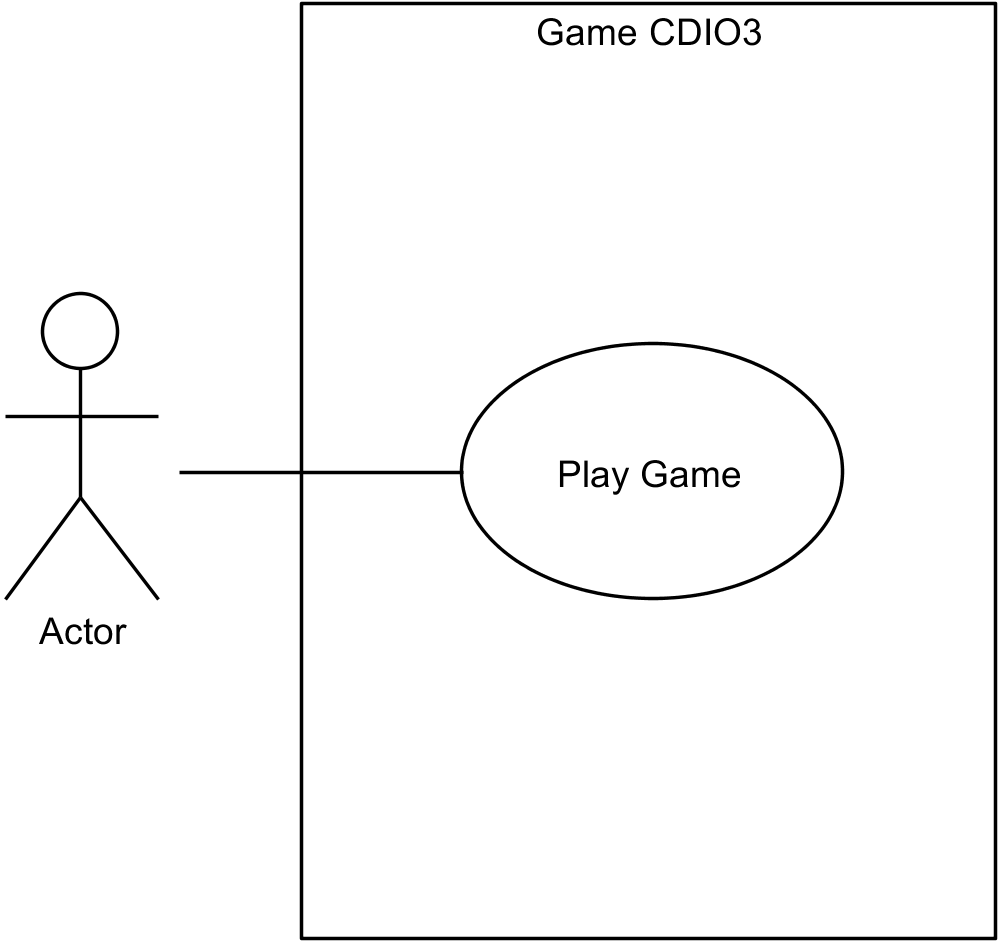
\includegraphics[width=8cm]{graphics/usecases/UseCase1.png}
        \caption{Use case diagram}
        \label{fig:use_case_diagram}
    \end{center}
\end{figure}

\pagebreak
\section{Domænemodel}